\begin{figure}[H]
     \centering
     %Drift angle
     \begin{subfigure}[b]{0.32\textwidth}
         \centering
        \includesvg[width=1.2 in]{figures/results_wPCC_VCT.drift_angle_X.svg}
        \caption{X for drift angle tests.}
        \label{fig:drift_angle_X_wPCC}
     \end{subfigure}
     \hfill
     \begin{subfigure}[b]{0.32\textwidth}
         \centering
         \includesvg{figures/results_wPCC_VCT.drift_angle_Y.svg}
        \caption{Y for drift angle tests.}
        \label{fig:drift_angle_Y_wPCC}
     \end{subfigure}
     \hfill
     \begin{subfigure}[b]{0.32\textwidth}
         \centering
         \includesvg{figures/results_wPCC_VCT.drift_angle_N.svg}
        \caption{N for drift angle tests.}
        \label{fig:drift_angle_N_wPCC}
     \end{subfigure}
    \vfill
    
     %Circle
     \begin{subfigure}[b]{0.32\textwidth}
         \centering
         \includesvg{figures/results_wPCC_VCT.circle_X.svg}
        \caption{X for circle tests.}
        \label{fig:circle_X_wPCC}
     \end{subfigure}
     \hfill
     \begin{subfigure}[b]{0.32\textwidth}
         \centering
         \includesvg{figures/results_wPCC_VCT.circle_Y.svg}
        \caption{Y for circle tests.}
        \label{fig:circle_Y_wPCC}
     \end{subfigure}
     \hfill
     \begin{subfigure}[b]{0.32\textwidth}
         \centering
         \includesvg{figures/results_wPCC_VCT.circle_N.svg}
        \caption{N for circle tests.}
        \label{fig:circle_N_wPCC}
     \end{subfigure}

    \vfill
    %rudder angle
     \begin{subfigure}[b]{0.32\textwidth}
         \centering
         \includesvg{figures/results_wPCC_VCT.rudder_angle_X.svg}
        \caption{X for rudder angle tests.}
        \label{fig:rudder_angle_X_wPCC}
     \end{subfigure}
     \hfill
     \begin{subfigure}[b]{0.32\textwidth}
         \centering
         \includesvg{figures/results_wPCC_VCT.rudder_angle_Y.svg}
        \caption{Y for rudder angle tests.}
        \label{fig:rudder_angle_Y_wPCC}
     \end{subfigure}
     \hfill
     \begin{subfigure}[b]{0.32\textwidth}
         \centering
         \includesvg{figures/results_wPCC_VCT.rudder_angle_N.svg}
        \caption{N for rudder angle tests.}
        \label{fig:rudder_angle_N_wPCC}
     \end{subfigure}

     \vfill
     %Thrust variation
     \begin{subfigure}[b]{0.32\textwidth}
         \centering
         \includesvg{figures/results_wPCC_VCT.thrust_variation_X.svg}
        \caption{Thrust variation X.}
        \label{fig:Thrust variation_X_wPCC}
     \end{subfigure}
     \hfill
     \begin{subfigure}[b]{0.32\textwidth}
         \centering
         \includesvg{figures/results_wPCC_VCT.thrust_variation_Y.svg}
        \caption{Thrust variation Y.}
        \label{fig:Thrust variation_Y_wPCC}
     \end{subfigure}
     \hfill
     \begin{subfigure}[b]{0.32\textwidth}
         \centering
         \includesvg{figures/results_wPCC_VCT.thrust_variation_N.svg}
        \caption{Thrust variation N.}
        \label{fig:Thrust variation_N_wPCC}
     \end{subfigure}
     
    \caption{Forces on the wPCC analyzed by VCT (dots) and predictions from the identified model (lines).}
    \label{fig:VCT_wPCC}
\end{figure}

\noindent The identified wPCC model fitted the VCT data well, as shown in \autoref{fig:VCT_wPCC}. 
It can be seen that the hull creates almost no damping yawing moment $N_H$ for smaller drift angles, as shown in \autoref{fig:drift_angle_N_wPCC}. This means that most of the total yawing moment is instead created by the inviscid Munk moment. The rudders are thus the main contributors to the viscous yawing moment. However, a non-linear viscous contribution is present in $N_H$ for larger drift angles. 

The coupling terms $Y_{vrr}$,$Y_{vvr}$,$N_{vrr}$, and $N_{vvr}$ in the hull force model (\autoref{eq:XYN_H_prime}) were fitted from the circle and drift variations. These coupling terms are important as shown by the comparison with/without them in \autoref{fig:circle_drift_wPCC}.


%Circle + drift
\begin{figure}[h]
     \centering
     \begin{subfigure}[b]{0.49\textwidth}
         \centering
         \includesvg{figures/results_wPCC_VCT.Y_H.svg}
        \caption{Sway force.}
        \label{fig:circle_drift_Y_H_wPCC}
     \end{subfigure}
     \hfill
     \begin{subfigure}[b]{0.49\textwidth}
         \centering
         \includesvg{figures/results_wPCC_VCT.Y_H_no_coupling.svg}
        \caption{Sway force no coupling.}
        \label{fig:circle_drift_Y_H_no_coupling_wPCC}
     \end{subfigure}

     \vfill
     \begin{subfigure}[b]{0.49\textwidth}
         \centering
         \includesvg{figures/results_wPCC_VCT.N_H.svg}
        \caption{Yawing moment.}
        \label{fig:circle_drift_N_H_wPCC}
     \end{subfigure}
     \hfill
     \begin{subfigure}[b]{0.49\textwidth}
         \centering
         \includesvg{figures/results_wPCC_VCT.N_H_no_coupling.svg}
        \caption{Yawing moment no coupling.}
        \label{fig:circle_drift_N_H_no_coupling_wPCC}
     \end{subfigure}
     
    \caption{wPCC hull forces during the circle and drift variations with/without the coupling terms, VCT (dots), fitted model (surface).}
    \label{fig:circle_drift_wPCC}
\end{figure}






%The flow from the port daggerboard was also observed to reach the starboard rudder for a 15-degree drift angle, as shown in Fig.\ref{fig:wpcc_drift_flow}. 
%\begin{figure}[h!]
%    \centering
%    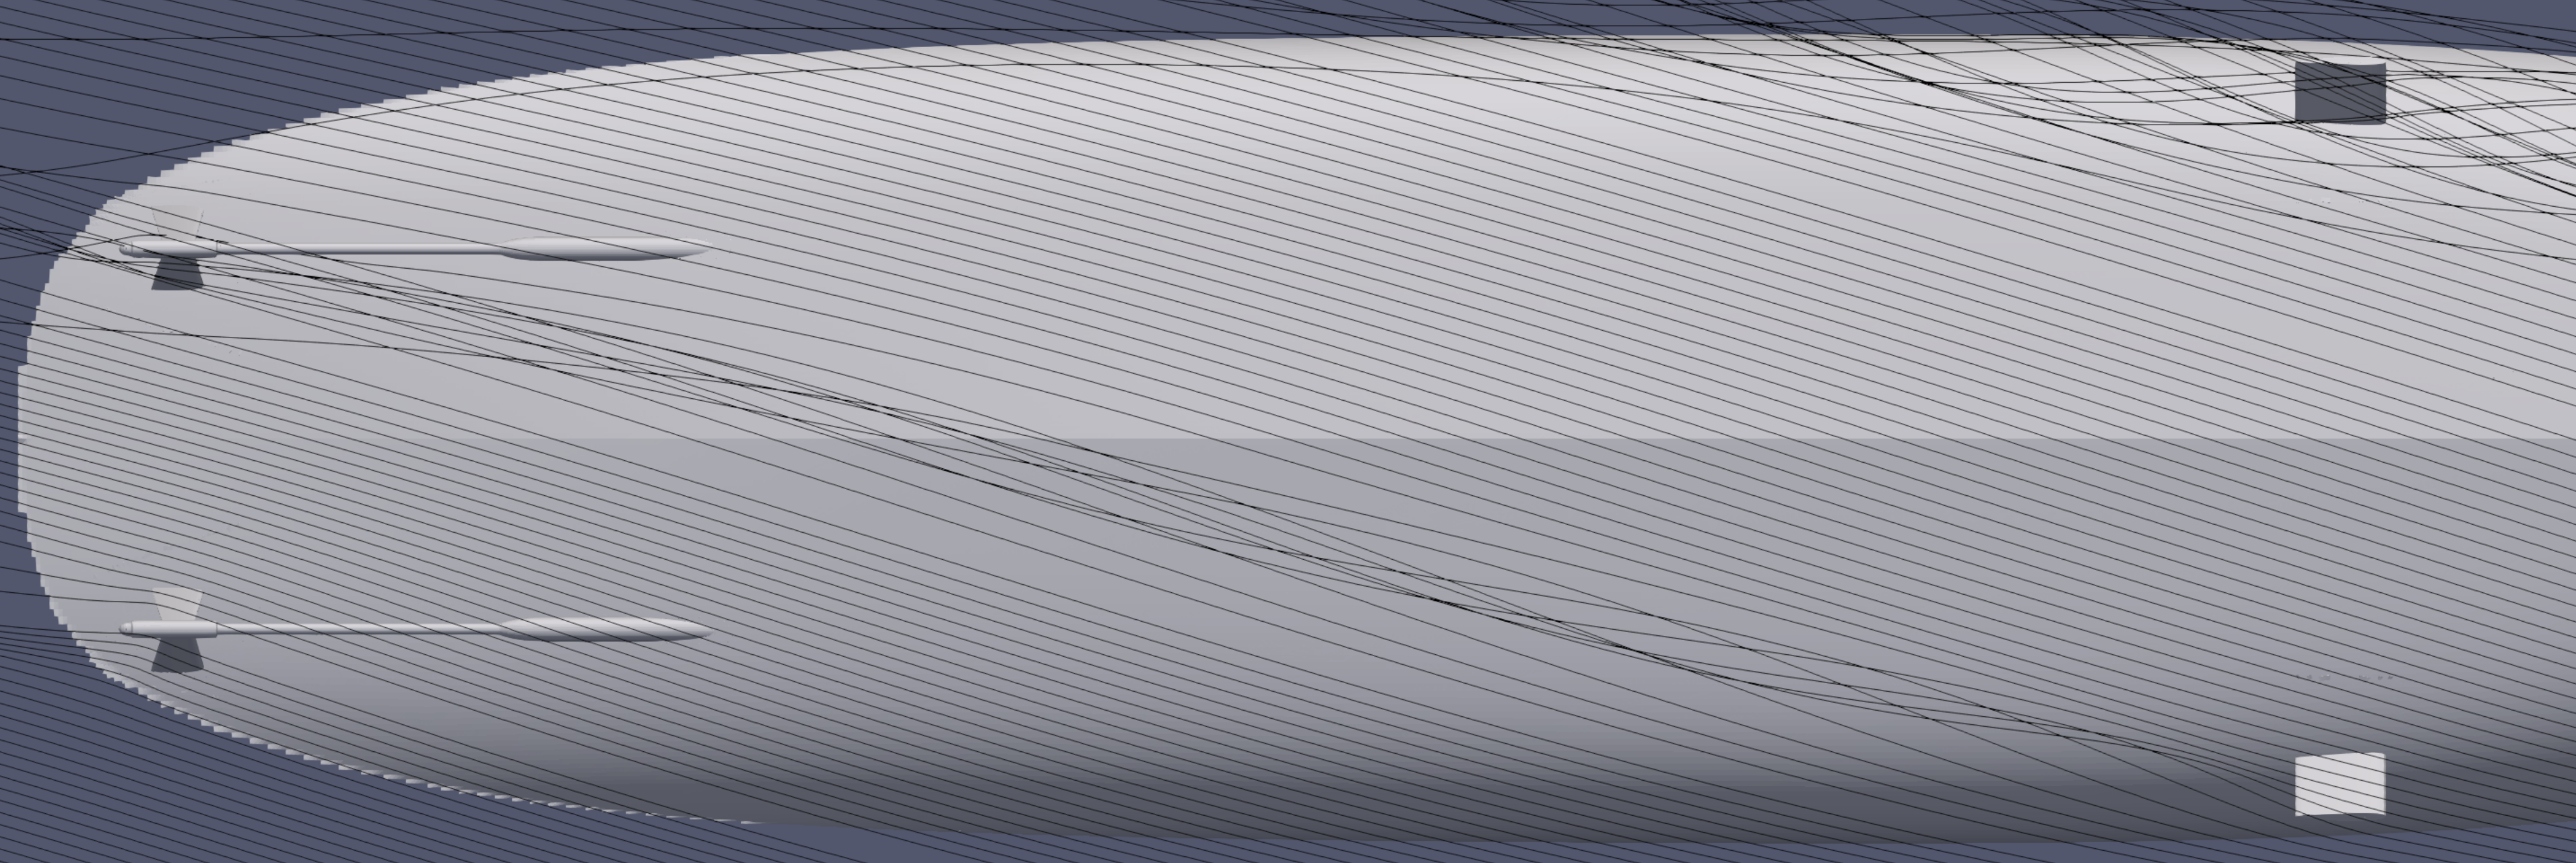
\includegraphics[width=5in]{figures/paraview_drift_15.png}
%    \caption{Flows at the wPCC bottom for VCT at 15 degrees drifting}
%    \label{fig:wpcc_drift_flow}
%\end{figure}
% \begin{figure}[h]
%      \centering
%      %Drift angle
%      \begin{subfigure}[b]{0.325\textwidth}
%          \centering
%          \includesvg{figures/results_wPCC_VCT.drift_angle_X.svg}
%         \caption{X at various drift angles}
%         \label{fig:drift_angle_X_wPCC}
%      \end{subfigure}
%      \hfill
%      \begin{subfigure}[b]{0.325\textwidth}
%          \centering
%          \includesvg{figures/results_wPCC_VCT.drift_angle_Y.svg}
%         \caption{Y at various drift angles}
%         \label{fig:drift_angle_Y_wPCC}
%      \end{subfigure}
%      \hfill
%      \begin{subfigure}[b]{0.325\textwidth}
%          \centering
%          \includesvg{figures/results_wPCC_VCT.drift_angle_N.svg}
%         \caption{N at various drift angles}
%         \label{fig:drift_angle_N_wPCC}
%      \end{subfigure}
%     % \vfill
    
%      %Circle
%      \begin{subfigure}[b]{0.325\textwidth}
%          \centering
%          \includesvg{figures/results_wPCC_VCT.circle_X.svg}
%         \caption{X at various circle angles}
%         \label{fig:circle_X_wPCC}
%      \end{subfigure}
%      \hfill
%      \begin{subfigure}[b]{0.325\textwidth}
%          \centering
%          \includesvg{figures/results_wPCC_VCT.circle_Y.svg}
%         \caption{Y at various circle angles}
%         \label{fig:circle_Y_wPCC}
%      \end{subfigure}
%      \hfill
%      \begin{subfigure}[b]{0.325\textwidth}
%          \centering
%          \includesvg{figures/results_wPCC_VCT.circle_N.svg}
%         \caption{N at various circle angles}
%         \label{fig:circle_N_wPCC}
%      \end{subfigure}

%     % \vfill
%     %rudder angle
%      \begin{subfigure}[b]{0.325\textwidth}
%          \centering
%          \includesvg{figures/results_wPCC_VCT.rudder_angle_X.svg}
%         \caption{X at various rudder angles}
%         \label{fig:rudder_angle_X_wPCC}
%      \end{subfigure}
%      \hfill
%      \begin{subfigure}[b]{0.325\textwidth}
%          \centering
%          \includesvg{figures/results_wPCC_VCT.rudder_angle_Y.svg}
%         \caption{Y at various rudder angles}
%         \label{fig:rudder_angle_Y_wPCC}
%      \end{subfigure}
%      \hfill
%      \begin{subfigure}[b]{0.325\textwidth}
%          \centering
%          \includesvg{figures/results_wPCC_VCT.rudder_angle_N.svg}
%         \caption{N at various rudder angles}
%         \label{fig:rudder_angle_N_wPCC}
%      \end{subfigure}

%      % \vfill
%      %Thrust variation
%      \begin{subfigure}[b]{0.325\textwidth}
%          \centering
%          \includesvg{figures/results_wPCC_VCT.thrust_variation_X.svg}
%         \caption{X at various thrust}
%         \label{fig:Thrust variation_X_wPCC}
%      \end{subfigure}
%      \hfill
%      \begin{subfigure}[b]{0.325\textwidth}
%          \centering
%          \includesvg{figures/results_wPCC_VCT.thrust_variation_Y.svg}
%         \caption{Y at various thrust}
%         \label{fig:Thrust variation_Y_wPCC}
%      \end{subfigure}
%      \hfill
%      \begin{subfigure}[b]{0.325\textwidth}
%          \centering
%          \includesvg{figures/results_wPCC_VCT.thrust_variation_N.svg}
%         \caption{N at various thrust}
%         \label{fig:Thrust variation_N_wPCC}
%      \end{subfigure}
     
%     \caption{Forces on the wPCC analyzed by VCT (dots) and predictions from the identified model (lines).}
%     \label{fig:VCT_wPCC}
% \end{figure}

%%%%%%%%%%%%%%%%%%%%%%%% Coupling vs uncoupling results %%%%%%%%%%%%%%%%

%Circle + drift
% \begin{figure}[h]
%      \centering
%      \begin{subfigure}[c]{.495\linewidth}
%          \centering
%          \includesvg[width=3.8in, height = 4in]{figures/results_wPCC_VCT.Y_H.svg}
%         \caption{Sway force.}
%         \label{fig:circle_drift_Y_H_wPCC}
%      \end{subfigure}
% %     \hfill
%      \begin{subfigure}[c]{0.495\linewidth}
%          \centering
%          \includesvg[width=3.8in, height = 4in]{figures/results_wPCC_VCT.Y_H_no_coupling.svg}
%         \caption{Sway force no coupling.}
%         \label{fig:circle_drift_Y_H_no_coupling_wPCC}
%      \end{subfigure}

%      \vfill
%      \begin{subfigure}[c]{0.495\linewidth}
%          \centering
%          \includesvg[width=3.8in, height = 4in]{figures/results_wPCC_VCT.N_H.svg}
%         \caption{Yawing moment.}
%         \label{fig:circle_drift_N_H_wPCC}
%      \end{subfigure}
% %     \hfill
%      \begin{subfigure}[c]{0.495\linewidth}
%          \centering
%          \includesvg[width=3.8in, height = 4in]{figures/results_wPCC_VCT.N_H_no_coupling.svg}
%         \caption{Yawing moment no coupling.}
%         \label{fig:circle_drift_N_H_no_coupling_wPCC}
%      \end{subfigure}     
%     \caption{wPCC hull forces during the circle and drift variations with/without the coupling terms, VCT (dots), fitted model (surface).}
%     \label{fig:circle_drift_wPCC}
% \end{figure}

